% Options for packages loaded elsewhere
\PassOptionsToPackage{unicode}{hyperref}
\PassOptionsToPackage{hyphens}{url}
%
\documentclass[
]{article}
\usepackage{lmodern}
\usepackage{amsmath}
\usepackage{ifxetex,ifluatex}
\ifnum 0\ifxetex 1\fi\ifluatex 1\fi=0 % if pdftex
  \usepackage[T1]{fontenc}
  \usepackage[utf8]{inputenc}
  \usepackage{textcomp} % provide euro and other symbols
  \usepackage{amssymb}
\else % if luatex or xetex
  \usepackage{unicode-math}
  \defaultfontfeatures{Scale=MatchLowercase}
  \defaultfontfeatures[\rmfamily]{Ligatures=TeX,Scale=1}
\fi
% Use upquote if available, for straight quotes in verbatim environments
\IfFileExists{upquote.sty}{\usepackage{upquote}}{}
\IfFileExists{microtype.sty}{% use microtype if available
  \usepackage[]{microtype}
  \UseMicrotypeSet[protrusion]{basicmath} % disable protrusion for tt fonts
}{}
\makeatletter
\@ifundefined{KOMAClassName}{% if non-KOMA class
  \IfFileExists{parskip.sty}{%
    \usepackage{parskip}
  }{% else
    \setlength{\parindent}{0pt}
    \setlength{\parskip}{6pt plus 2pt minus 1pt}}
}{% if KOMA class
  \KOMAoptions{parskip=half}}
\makeatother
\usepackage{xcolor}
\IfFileExists{xurl.sty}{\usepackage{xurl}}{} % add URL line breaks if available
\IfFileExists{bookmark.sty}{\usepackage{bookmark}}{\usepackage{hyperref}}
\hypersetup{
  pdftitle={Analyzing GazePoint Data with GazeR},
  pdfauthor={Jason Geller},
  hidelinks,
  pdfcreator={LaTeX via pandoc}}
\urlstyle{same} % disable monospaced font for URLs
\usepackage[margin=1in]{geometry}
\usepackage{color}
\usepackage{fancyvrb}
\newcommand{\VerbBar}{|}
\newcommand{\VERB}{\Verb[commandchars=\\\{\}]}
\DefineVerbatimEnvironment{Highlighting}{Verbatim}{commandchars=\\\{\}}
% Add ',fontsize=\small' for more characters per line
\usepackage{framed}
\definecolor{shadecolor}{RGB}{248,248,248}
\newenvironment{Shaded}{\begin{snugshade}}{\end{snugshade}}
\newcommand{\AlertTok}[1]{\textcolor[rgb]{0.94,0.16,0.16}{#1}}
\newcommand{\AnnotationTok}[1]{\textcolor[rgb]{0.56,0.35,0.01}{\textbf{\textit{#1}}}}
\newcommand{\AttributeTok}[1]{\textcolor[rgb]{0.77,0.63,0.00}{#1}}
\newcommand{\BaseNTok}[1]{\textcolor[rgb]{0.00,0.00,0.81}{#1}}
\newcommand{\BuiltInTok}[1]{#1}
\newcommand{\CharTok}[1]{\textcolor[rgb]{0.31,0.60,0.02}{#1}}
\newcommand{\CommentTok}[1]{\textcolor[rgb]{0.56,0.35,0.01}{\textit{#1}}}
\newcommand{\CommentVarTok}[1]{\textcolor[rgb]{0.56,0.35,0.01}{\textbf{\textit{#1}}}}
\newcommand{\ConstantTok}[1]{\textcolor[rgb]{0.00,0.00,0.00}{#1}}
\newcommand{\ControlFlowTok}[1]{\textcolor[rgb]{0.13,0.29,0.53}{\textbf{#1}}}
\newcommand{\DataTypeTok}[1]{\textcolor[rgb]{0.13,0.29,0.53}{#1}}
\newcommand{\DecValTok}[1]{\textcolor[rgb]{0.00,0.00,0.81}{#1}}
\newcommand{\DocumentationTok}[1]{\textcolor[rgb]{0.56,0.35,0.01}{\textbf{\textit{#1}}}}
\newcommand{\ErrorTok}[1]{\textcolor[rgb]{0.64,0.00,0.00}{\textbf{#1}}}
\newcommand{\ExtensionTok}[1]{#1}
\newcommand{\FloatTok}[1]{\textcolor[rgb]{0.00,0.00,0.81}{#1}}
\newcommand{\FunctionTok}[1]{\textcolor[rgb]{0.00,0.00,0.00}{#1}}
\newcommand{\ImportTok}[1]{#1}
\newcommand{\InformationTok}[1]{\textcolor[rgb]{0.56,0.35,0.01}{\textbf{\textit{#1}}}}
\newcommand{\KeywordTok}[1]{\textcolor[rgb]{0.13,0.29,0.53}{\textbf{#1}}}
\newcommand{\NormalTok}[1]{#1}
\newcommand{\OperatorTok}[1]{\textcolor[rgb]{0.81,0.36,0.00}{\textbf{#1}}}
\newcommand{\OtherTok}[1]{\textcolor[rgb]{0.56,0.35,0.01}{#1}}
\newcommand{\PreprocessorTok}[1]{\textcolor[rgb]{0.56,0.35,0.01}{\textit{#1}}}
\newcommand{\RegionMarkerTok}[1]{#1}
\newcommand{\SpecialCharTok}[1]{\textcolor[rgb]{0.00,0.00,0.00}{#1}}
\newcommand{\SpecialStringTok}[1]{\textcolor[rgb]{0.31,0.60,0.02}{#1}}
\newcommand{\StringTok}[1]{\textcolor[rgb]{0.31,0.60,0.02}{#1}}
\newcommand{\VariableTok}[1]{\textcolor[rgb]{0.00,0.00,0.00}{#1}}
\newcommand{\VerbatimStringTok}[1]{\textcolor[rgb]{0.31,0.60,0.02}{#1}}
\newcommand{\WarningTok}[1]{\textcolor[rgb]{0.56,0.35,0.01}{\textbf{\textit{#1}}}}
\usepackage{longtable,booktabs}
\usepackage{calc} % for calculating minipage widths
% Correct order of tables after \paragraph or \subparagraph
\usepackage{etoolbox}
\makeatletter
\patchcmd\longtable{\par}{\if@noskipsec\mbox{}\fi\par}{}{}
\makeatother
% Allow footnotes in longtable head/foot
\IfFileExists{footnotehyper.sty}{\usepackage{footnotehyper}}{\usepackage{footnote}}
\makesavenoteenv{longtable}
\usepackage{graphicx}
\makeatletter
\def\maxwidth{\ifdim\Gin@nat@width>\linewidth\linewidth\else\Gin@nat@width\fi}
\def\maxheight{\ifdim\Gin@nat@height>\textheight\textheight\else\Gin@nat@height\fi}
\makeatother
% Scale images if necessary, so that they will not overflow the page
% margins by default, and it is still possible to overwrite the defaults
% using explicit options in \includegraphics[width, height, ...]{}
\setkeys{Gin}{width=\maxwidth,height=\maxheight,keepaspectratio}
% Set default figure placement to htbp
\makeatletter
\def\fps@figure{htbp}
\makeatother
\setlength{\emergencystretch}{3em} % prevent overfull lines
\providecommand{\tightlist}{%
  \setlength{\itemsep}{0pt}\setlength{\parskip}{0pt}}
\setcounter{secnumdepth}{-\maxdimen} % remove section numbering
\ifluatex
  \usepackage{selnolig}  % disable illegal ligatures
\fi

\title{Analyzing GazePoint Data with GazeR}
\author{Jason Geller}
\date{2021-04-27 12:02:03}

\begin{document}
\maketitle

In this vignette I am going to show you how to read in a GazePoint data
file along with some behavioral data and use \texttt{gazeR} to
preprocess the data.

Special thanks to Matthew K Robinson (Twitter:@matthewkrobinson) for
letting me use some data from an auditory oddball task he conducted on
himself (we do what we have to do as a researcher :D): see Tweet below.

i'm just a guy, running himself through auditory oddball tasks on his
new eye-tracker, asking it to love him back. pic.twitter.com/wPb97MZuNF

--- Matthew K. Robison (@matthewkrobison) April 19, 2021

To get started, we need to load in some important packages and read in
the GP data files.

\hypertarget{load-packages}{%
\section{Load Packages}\label{load-packages}}

\begin{Shaded}
\begin{Highlighting}[]
\FunctionTok{library}\NormalTok{(tidyverse)}
\CommentTok{\#install\_github("dmirman/gazer")}
\FunctionTok{library}\NormalTok{(gazer)}
\FunctionTok{library}\NormalTok{(data.table)}
\FunctionTok{library}\NormalTok{(here)}
\NormalTok{remotes}\SpecialCharTok{::}\FunctionTok{install\_github}\NormalTok{(}\StringTok{"tmalsburg/saccades/saccades"}\NormalTok{, }\AttributeTok{dependencies=}\ConstantTok{TRUE}\NormalTok{)}
\FunctionTok{library}\NormalTok{(saccades)}
\end{Highlighting}
\end{Shaded}

\hypertarget{read-data}{%
\section{Read Data}\label{read-data}}

\begin{Shaded}
\begin{Highlighting}[]
\NormalTok{pd }\OtherTok{\textless{}{-}} \FunctionTok{fread}\NormalTok{(here}\SpecialCharTok{::}\FunctionTok{here}\NormalTok{(}\StringTok{\textquotesingle{}oddball\_eye\_13.tsv\textquotesingle{}}\NormalTok{)) }\CommentTok{\# eye data }
\NormalTok{bs}\OtherTok{\textless{}{-}}\FunctionTok{fread}\NormalTok{(here}\SpecialCharTok{::}\FunctionTok{here}\NormalTok{(}\StringTok{\textquotesingle{}oddball\_13.tsv\textquotesingle{}}\NormalTok{)) }\CommentTok{\# behave data}

\FunctionTok{head}\NormalTok{(pd)}
\end{Highlighting}
\end{Shaded}

\begin{verbatim}
##      CNT     TIME    TIME_TICK    FPOGX     FPOGY    FPOGS   FPOGD FPOGID FPOGV
## 1: 77433 1251.964 102150661899 -4.40518 -13.98604 1251.883 0.08093   1917     1
## 2: 77434 1251.980 102150821625 -4.39508 -13.95200 1251.883 0.09692   1917     1
## 3: 77435 1251.996 102150983307 -4.36427 -13.84678 1251.883 0.09692   1917     0
## 4: 77436 1252.013 102151149297 -4.40694 -13.99395 1251.883 0.09692   1917     0
## 5: 77437 1252.028 102151307171 -4.42096 -14.04383 1251.883 0.09692   1917     0
## 6: 77438 1252.045 102151469190 -4.40730 -14.00445 1251.883 0.09692   1917     0
##      LPOGX   LPOGY LPOGV    RPOGX     RPOGY RPOGV    BPOGX     BPOGY BPOGV
## 1: 0.71795 0.50537     1 -9.38697 -28.00086     1 -4.33451 -13.74775     1
## 2: 0.71795 0.50537     1 -9.38697 -28.00086     1 -4.33451 -13.74775     1
## 3: 0.70711 0.51136     1 -9.14516 -27.18135     1 -4.21902 -13.33500     1
## 4: 0.70151 0.43055     1 -9.60071 -28.71280     1 -4.44960 -14.14113     1
## 5: 0.70270 0.42562     1 -9.60071 -28.71280     1 -4.44900 -14.14359     1
## 6: 0.69827 0.43625     1 -9.34484 -27.89350     1 -4.32329 -13.72862     1
##       LPCX    LPCY      LPD     LPS LPV    RPCX    RPCY      RPD RPS RPV
## 1: 0.34860 0.59214 25.23420 0.83829   1 0.64310 0.60511 28.49240   1   1
## 2: 0.34860 0.59216 25.27127 0.83829   1 0.64314 0.60509 28.33148   1   1
## 3: 0.34845 0.59234 25.09805 0.83829   1 0.64293 0.60517 28.69580   1   1
## 4: 0.34846 0.59237 25.15947 0.83829   1 0.64286 0.60519 28.47081   1   1
## 5: 0.34838 0.59240 25.32249 0.84484   1 0.64285 0.60518 28.46784   1   1
## 6: 0.34830 0.59240 25.07680 0.85139   1 0.64269 0.60527 28.50588   1   1
##       LEYEX    LEYEY   LEYEZ LPUPILD LPUPILV   REYEX    REYEY   REYEZ RPUPILD
## 1: -0.03362 -0.01726 0.56538 0.00455       1 0.03052 -0.01989 0.57411 0.00512
## 2: -0.03438 -0.01769 0.57821 0.00451       1 0.03056 -0.01997 0.57644 0.00513
## 3: -0.03438 -0.01769 0.57821 0.00449       1 0.03056 -0.01997 0.57644 0.00510
## 4: -0.03438 -0.01769 0.57821 0.00451       1 0.03056 -0.01997 0.57644 0.00509
## 5: -0.03501 -0.01795 0.58649 0.00448       1 0.03130 -0.02049 0.59132 0.00509
## 6: -0.03501 -0.01795 0.58649 0.00450       1 0.03130 -0.02049 0.59132 0.00508
##    RPUPILV      CX      CY CS BKID BKDUR BKPMIN    LPMM LPMMV    RPMM RPMMV
## 1:       1 0.33333 0.33333  0    0     0     20 4.54567     1 5.11614     1
## 2:       1 0.33333 0.33333  0    0     0     20 4.51065     1 5.12683     1
## 3:       1 0.33333 0.33333  0    0     0     20 4.48607     1 5.10490     1
## 4:       1 0.33333 0.33333  0    0     0     20 4.50748     1 5.09460     1
## 5:       1 0.33333 0.33333  0    0     0     20 4.47957     1 5.08827     1
## 6:       1 0.33333 0.33333  0    0     0     20 4.50258     1 5.07552     1
##     DIAL DIALV GSR GSRV HR HRV HRP TTL0 TTL1 TTLV            USER
## 1: 0.088     1   0    0  0   0 454   -1   -1    0               0
## 2: 0.088     1   0    0  0   0 484   -1   -1    0 STARTEXPERIMENT
## 3: 0.088     1   0    0  0   0 456   -1   -1    0 STARTEXPERIMENT
## 4: 0.088     1   0    0  0   0 451   -1   -1    0           START
## 5: 0.088     1   0    0  0   0 482   -1   -1    0           START
## 6: 0.088     1   0    0  0   0 454   -1   -1    0           START
\end{verbatim}

\begin{Shaded}
\begin{Highlighting}[]
\FunctionTok{head}\NormalTok{(bs)}
\end{Highlighting}
\end{Shaded}

\begin{verbatim}
##    subject trial tone   rt response
## 1:      13     1   lo 2113     None
## 2:      13     2   lo 2102     None
## 3:      13     3   lo 2107     None
## 4:      13     4   lo 2108     None
## 5:      13     5   lo 2107     None
## 6:      13     6   lo 2103     None
\end{verbatim}

What we are going to do is run the GazePoint file through the
\texttt{merge\_gazepoint} function. The function below takes a list of
files called file\_list and merges all the files together, appends a
subject column, creates a trial column using the USER column (GazePoint
only allows messages through this channel), creates a time variable (in
milliseconds). In the \texttt{merge\_gazepoint} function the
\texttt{trail\_msg} argument requires users to denote a message used in
the USER column that references the start of the trial--in our case the
\texttt{START} message denotes the start of a new trial. This is a
solution by Matt Robinson, but there are other ways one could extract
the trial number. What I have done in the past is append a message with
the trial iteration (e.g., START\_1) in Python and use the
\texttt{separate} function to get the trial number.

\begin{Shaded}
\begin{Highlighting}[]
\CommentTok{\# A "monocular mean" averages both eyes together. If data is available in just}
\CommentTok{\# one eye, use the available value as the mean, unless we need\_both is TRUE.}
\CommentTok{\#\textquotesingle{} @param x1 pupil left}
\CommentTok{\#\textquotesingle{} @param x2 pupil right}
\CommentTok{\#\textquotesingle{} @return vector with monocular mean values}
\NormalTok{compute\_monocular\_mean }\OtherTok{\textless{}{-}} \ControlFlowTok{function}\NormalTok{(x1, x2) \{}
\NormalTok{  xm }\OtherTok{\textless{}{-}} \FunctionTok{rowMeans}\NormalTok{(}\FunctionTok{cbind}\NormalTok{(x1, x2), }\AttributeTok{na.rm =} \ConstantTok{TRUE}\NormalTok{)}
  \CommentTok{\# NaN =\textgreater{} NA}
  \FunctionTok{ifelse}\NormalTok{(}\FunctionTok{is.nan}\NormalTok{(xm), }\ConstantTok{NA}\NormalTok{, xm)}
\NormalTok{\}}


\CommentTok{\# function for processing GazePoint data}
\NormalTok{merge\_gazepoint }\OtherTok{\textless{}{-}} \ControlFlowTok{function}\NormalTok{ (file\_list, }\AttributeTok{trial\_msg =} \StringTok{"START"}\NormalTok{)\{}
  \CommentTok{\#file list is path to .xls files}
  \CommentTok{\#vroom is faster}
  \FunctionTok{library}\NormalTok{(data.table)}
  
\NormalTok{  file\_ids}\OtherTok{=}\FunctionTok{str\_replace\_all}\NormalTok{(}\FunctionTok{basename}\NormalTok{(file\_list),}\StringTok{"([:alpha:]|[:punct:])"}\NormalTok{,}\StringTok{""}\NormalTok{) }\CommentTok{\# remove everything but numeric values}
                   
\NormalTok{  data }\OtherTok{\textless{}{-}} \FunctionTok{map2}\NormalTok{(file\_list, file\_ids, }\SpecialCharTok{\textasciitilde{}}\FunctionTok{fread}\NormalTok{(.x) }\SpecialCharTok{\%\textgreater{}\%} 
    \FunctionTok{mutate}\NormalTok{(}\AttributeTok{id =}\NormalTok{ .y))  }\SpecialCharTok{\%\textgreater{}\%} 
    \FunctionTok{bind\_rows}\NormalTok{()}

  
\NormalTok{  d }\OtherTok{=}\NormalTok{ data }\SpecialCharTok{\%\textgreater{}\%}
\NormalTok{    dplyr}\SpecialCharTok{::}\FunctionTok{rowwise}\NormalTok{() }\SpecialCharTok{\%\textgreater{}\%}
\NormalTok{    dplyr}\SpecialCharTok{::}\FunctionTok{mutate}\NormalTok{(}\AttributeTok{pupil=}\FunctionTok{compute\_monocular\_mean}\NormalTok{(RPMM, LPMM)) }\SpecialCharTok{\%\textgreater{}\%} \CommentTok{\# average both eyes}
\NormalTok{             dplyr}\SpecialCharTok{::}\FunctionTok{ungroup}\NormalTok{() }\SpecialCharTok{\%\textgreater{}\%}
\NormalTok{           dplyr}\SpecialCharTok{::}\FunctionTok{mutate}\NormalTok{(}\AttributeTok{pupil =} \FunctionTok{ifelse}\NormalTok{(RPMMV }\SpecialCharTok{==} \DecValTok{0}\SpecialCharTok{|}\NormalTok{LPMMV }\SpecialCharTok{==} \DecValTok{0}\NormalTok{, }\DecValTok{0}\NormalTok{, pupil),  }\CommentTok{\#missing data labeled as blinks}
         \AttributeTok{new\_trial =} \FunctionTok{ifelse}\NormalTok{(USER }\SpecialCharTok{==}\NormalTok{ trial\_msg }\SpecialCharTok{\&} \FunctionTok{lag}\NormalTok{(USER) }\SpecialCharTok{!=}\NormalTok{ trial\_msg, }\DecValTok{1}\NormalTok{, }\DecValTok{0}\NormalTok{), }\CommentTok{\# Label new trials}
         \AttributeTok{trial =} \FunctionTok{cumsum}\NormalTok{(new\_trial), }\CommentTok{\# Create a trial variable}
         \AttributeTok{time =} \FunctionTok{floor}\NormalTok{(TIME}\SpecialCharTok{*}\DecValTok{1000}\NormalTok{)) }\SpecialCharTok{\%\textgreater{}\%}
    \FunctionTok{group\_by}\NormalTok{(trial) }\SpecialCharTok{\%\textgreater{}\%}
\NormalTok{    dplyr}\SpecialCharTok{::}\FunctionTok{mutate}\NormalTok{(}\AttributeTok{time=}\NormalTok{time }\SpecialCharTok{{-}} \FunctionTok{min}\NormalTok{(time)) }\SpecialCharTok{\%\textgreater{}\%}
    \FunctionTok{ungroup}\NormalTok{() }\SpecialCharTok{\%\textgreater{}\%}
\NormalTok{  dplyr}\SpecialCharTok{::}\FunctionTok{select}\NormalTok{(id, time,trial,pupil,BPOGX, BPOGY, USER) }\SpecialCharTok{\%\textgreater{}\%}
\NormalTok{    dplyr}\SpecialCharTok{::}\FunctionTok{rename}\NormalTok{(}\StringTok{"message"} \OtherTok{=} \StringTok{"USER"}\NormalTok{, }\StringTok{"subject"}\OtherTok{=} \StringTok{"id"}\NormalTok{, }\StringTok{"x"} \OtherTok{=} \StringTok{"BPOGX"}\NormalTok{, }\StringTok{"y"} \OtherTok{=} \StringTok{"BPOGY"}\NormalTok{) }\SpecialCharTok{\%\textgreater{}\%} 
\NormalTok{    dplyr}\SpecialCharTok{::}\FunctionTok{filter}\NormalTok{(trial }\SpecialCharTok{\textgreater{}} \DecValTok{0}\NormalTok{)}
  
  \FunctionTok{return}\NormalTok{(d)}
\NormalTok{\}}
\end{Highlighting}
\end{Shaded}

\hypertarget{merge-files-and-add-behav-data}{%
\section{Merge Files and add behav
data}\label{merge-files-and-add-behav-data}}

\begin{Shaded}
\begin{Highlighting}[]
\FunctionTok{setwd}\NormalTok{(}\FunctionTok{here}\NormalTok{()) }\CommentTok{\# setwd}

\NormalTok{gp\_file}\OtherTok{\textless{}{-}}\FunctionTok{list.files}\NormalTok{(here}\SpecialCharTok{::}\FunctionTok{here}\NormalTok{(), }\AttributeTok{pattern =} \StringTok{"eye\_13.tsv"}\NormalTok{) }\CommentTok{\# get files }

\FunctionTok{setwd}\NormalTok{(}\FunctionTok{here}\NormalTok{())}
      
\NormalTok{d}\OtherTok{=}\FunctionTok{merge\_gazepoint}\NormalTok{(gp\_file, }\AttributeTok{trial\_msg =} \StringTok{"START"}\NormalTok{)}

\NormalTok{d}\SpecialCharTok{$}\NormalTok{subject}\OtherTok{\textless{}{-}}\FunctionTok{as.numeric}\NormalTok{(d}\SpecialCharTok{$}\NormalTok{subject)}

\NormalTok{pdb }\OtherTok{\textless{}{-}} \FunctionTok{full\_join}\NormalTok{(bs, d)}

\NormalTok{pdb }\OtherTok{\textless{}{-}} \FunctionTok{as\_tibble}\NormalTok{(pdb)}

\NormalTok{pdb}
\end{Highlighting}
\end{Shaded}

\begin{verbatim}
## # A tibble: 73,724 x 10
##    subject trial tone     rt response  time pupil     x     y message
##      <dbl> <dbl> <chr> <int> <chr>    <dbl> <dbl> <dbl> <dbl> <chr>  
##  1      13     1 lo     2113 None         0  4.80 -4.45 -14.1 START  
##  2      13     1 lo     2113 None        16  4.78 -4.45 -14.1 START  
##  3      13     1 lo     2113 None        32  4.79 -4.32 -13.7 START  
##  4      13     1 lo     2113 None        48  4.80 -4.58 -14.5 START  
##  5      13     1 lo     2113 None        64  4.80 -4.58 -14.5 START  
##  6      13     1 lo     2113 None        81  4.79 -4.63 -14.7 START  
##  7      13     1 lo     2113 None        97  4.81 -4.42 -14.0 START  
##  8      13     1 lo     2113 None       113  4.80 -4.42 -14.0 TONE   
##  9      13     1 lo     2113 None       129  4.78 -4.23 -13.5 TONE   
## 10      13     1 lo     2113 None       145  4.77 -4.34 -13.8 TONE   
## # ... with 73,714 more rows
\end{verbatim}

\hypertarget{blinks}{%
\section{Blinks}\label{blinks}}

\hypertarget{finding-blinks}{%
\subsection{Finding Blinks}\label{finding-blinks}}

The GazePoint data does not indicate where blinks occurred. What we are
going to do is use the \texttt{blink\_detect} function in gazer. This
relies on the \texttt{saccades} package
(\url{https://github.com/tmalsburg/saccades}) which uses a velocity
based measure based on X,Y coordinates to find blinks. Once we find the
blinks we can change the pupil size at that time point as NA and
interpolate over it.

As a note, the GazePoint does not seem to sample consistently. In this
case, it samples every 16 or 17 ms. This is a problem for some other
blink detection measures (e.g., the noise based pupil function). One
soultion would be to downsample the data at the onset so there is
consistancy from sample to sample.

\begin{Shaded}
\begin{Highlighting}[]
\NormalTok{blinks\_merge}\OtherTok{\textless{}{-}} \FunctionTok{blink\_detect}\NormalTok{(pdb)}

\NormalTok{ blinks }\OtherTok{\textless{}{-}}\NormalTok{ blinks\_merge }\SpecialCharTok{\%\textgreater{}\%}
\NormalTok{        dplyr}\SpecialCharTok{::}\FunctionTok{group\_by}\NormalTok{(}\AttributeTok{grp =} \FunctionTok{cumsum}\NormalTok{(}\SpecialCharTok{!}\FunctionTok{is.na}\NormalTok{(startend))) }\SpecialCharTok{\%\textgreater{}\%}
\NormalTok{        dplyr}\SpecialCharTok{::}\FunctionTok{mutate}\NormalTok{(}\AttributeTok{Label =} \FunctionTok{replace}\NormalTok{(startend, }\FunctionTok{first}\NormalTok{(startend) }\SpecialCharTok{==} \StringTok{\textquotesingle{}start\textquotesingle{}}\NormalTok{, }\StringTok{\textquotesingle{}start\textquotesingle{}}\NormalTok{)) }\SpecialCharTok{\%\textgreater{}\%} \CommentTok{\#extends the start message forward until end message}
\NormalTok{        dplyr}\SpecialCharTok{::}\FunctionTok{ungroup}\NormalTok{() }\SpecialCharTok{\%\textgreater{}\%}
        \CommentTok{\# label blinks as 1}
\NormalTok{        dplyr}\SpecialCharTok{::}\FunctionTok{select}\NormalTok{(subject, trial, time, x, y, pupil, message, tone,  Label, }\SpecialCharTok{{-}}\NormalTok{grp)}
 
 
\NormalTok{ blinks\_data }\OtherTok{\textless{}{-}}\NormalTok{ blinks  }\SpecialCharTok{\%\textgreater{}\%}
\NormalTok{        dplyr}\SpecialCharTok{::}\FunctionTok{mutate}\NormalTok{(}\AttributeTok{blink=}\FunctionTok{ifelse}\NormalTok{(}\SpecialCharTok{!}\FunctionTok{is.na}\NormalTok{(Label), }\DecValTok{1}\NormalTok{, }\DecValTok{0}\NormalTok{), }\AttributeTok{pupil=}\FunctionTok{ifelse}\NormalTok{(blink}\SpecialCharTok{==}\DecValTok{1} \SpecialCharTok{|}\NormalTok{ pupil}\SpecialCharTok{==}\DecValTok{0}\NormalTok{, }\ConstantTok{NA}\NormalTok{, pupil))}\SpecialCharTok{\%\textgreater{}\%}
\NormalTok{        dplyr}\SpecialCharTok{::}\FunctionTok{ungroup}\NormalTok{()}\SpecialCharTok{\%\textgreater{}\%}
\NormalTok{        dplyr}\SpecialCharTok{::}\FunctionTok{select}\NormalTok{(subject, time, trial, pupil, x, y, trial, message, tone, blink, }\SpecialCharTok{{-}}\NormalTok{Label)}
\end{Highlighting}
\end{Shaded}

Here is a look at the trials containing blinks:

\begin{Shaded}
\begin{Highlighting}[]
\NormalTok{blinks\_data }\SpecialCharTok{\%\textgreater{}\%} 
  \FunctionTok{filter}\NormalTok{(blink}\SpecialCharTok{==}\DecValTok{1}\NormalTok{) }\SpecialCharTok{\%\textgreater{}\%}
  \FunctionTok{head}\NormalTok{()}\SpecialCharTok{\%\textgreater{}\%}
\NormalTok{  knitr}\SpecialCharTok{::}\FunctionTok{kable}\NormalTok{()}
\end{Highlighting}
\end{Shaded}

\begin{longtable}[]{@{}rrrrrrllr@{}}
\toprule
subject & time & trial & pupil & x & y & message & tone &
blink\tabularnewline
\midrule
\endhead
13 & 2167 & 10 & NA & 0.9364 & 1.95015 & POSTTONE & lo &
1\tabularnewline
13 & 2183 & 10 & NA & 0.9364 & 1.95015 & POSTTONE & lo &
1\tabularnewline
13 & 2199 & 10 & NA & 0.9364 & 1.95015 & POSTTONE & lo &
1\tabularnewline
13 & 2216 & 10 & NA & 0.9364 & 1.95015 & POSTTONE & lo &
1\tabularnewline
13 & 0 & 11 & NA & 0.9364 & 1.95015 & START & hi & 1\tabularnewline
13 & 16 & 11 & NA & 0.9364 & 1.95015 & START & hi & 1\tabularnewline
\bottomrule
\end{longtable}

\hypertarget{extending-blinks}{%
\subsection{Extending Blinks}\label{extending-blinks}}

I am extending blinks 100 ms forward and backward in time.

\hypertarget{interpolate-blinks}{%
\subsubsection{Interpolate Blinks}\label{interpolate-blinks}}

Here let's linearly interpolate the blinks and then smooth the data
using a 5-point moving average.

\begin{Shaded}
\begin{Highlighting}[]
\CommentTok{\# Smooth and Interpolate}
\NormalTok{smooth\_interp }\OtherTok{\textless{}{-}} \FunctionTok{smooth\_interpolate\_pupil}\NormalTok{(pup\_extend, }\AttributeTok{pupil=}\StringTok{"pupil"}\NormalTok{, }\AttributeTok{extendpupil=}\StringTok{"extendpupil"}\NormalTok{, }\AttributeTok{extendblinks=}\ConstantTok{TRUE}\NormalTok{, }\AttributeTok{step.first=}\StringTok{"smooth"}\NormalTok{, }\AttributeTok{maxgap=}\ConstantTok{Inf}\NormalTok{, }\AttributeTok{type=}\StringTok{"linear"}\NormalTok{, }\AttributeTok{hz=}\DecValTok{60}\NormalTok{, }\AttributeTok{n=}\DecValTok{5}\NormalTok{)}
\end{Highlighting}
\end{Shaded}

\hypertarget{plot-interpolated-trial}{%
\section{Plot Interpolated Trial}\label{plot-interpolated-trial}}

\begin{Shaded}
\begin{Highlighting}[]
\NormalTok{interp\_graph }\OtherTok{\textless{}{-}}\NormalTok{ smooth\_interp  }\SpecialCharTok{\%\textgreater{}\%}
\NormalTok{  dplyr}\SpecialCharTok{::}\FunctionTok{filter}\NormalTok{(trial}\SpecialCharTok{==}\StringTok{"400"}\NormalTok{)}

\NormalTok{bold }\OtherTok{\textless{}{-}} \FunctionTok{element\_text}\NormalTok{(}\AttributeTok{face =} \StringTok{"bold"}\NormalTok{, }\AttributeTok{color =} \StringTok{"black"}\NormalTok{, }\AttributeTok{size =} \DecValTok{14}\NormalTok{) }\CommentTok{\#axis bold}
\CommentTok{\#Graph interpolation}
\NormalTok{pup\_g}\OtherTok{\textless{}{-}} \FunctionTok{ggplot}\NormalTok{(interp\_graph, }\FunctionTok{aes}\NormalTok{(}\AttributeTok{x=}\NormalTok{ time, }\AttributeTok{y=}\NormalTok{ pupil)) }\SpecialCharTok{+} \FunctionTok{geom\_point}\NormalTok{()}\SpecialCharTok{+} \FunctionTok{geom\_line}\NormalTok{(}\AttributeTok{colour=}\StringTok{"black"}\NormalTok{) }\SpecialCharTok{+}
  \FunctionTok{geom\_line}\NormalTok{(}\FunctionTok{aes}\NormalTok{(}\AttributeTok{x=}\NormalTok{time, }\AttributeTok{y=}\NormalTok{pup\_interp), }\AttributeTok{colour=}\StringTok{"darkgreen"}\NormalTok{) }\SpecialCharTok{+} \FunctionTok{xlab}\NormalTok{(}\StringTok{"Time (ms)"}\NormalTok{) }\SpecialCharTok{+} \FunctionTok{ylab}\NormalTok{(}\StringTok{"Pupil Size (mm)"}\NormalTok{) }\SpecialCharTok{+} \FunctionTok{theme\_bw}\NormalTok{() }\SpecialCharTok{+} \FunctionTok{theme}\NormalTok{(}\AttributeTok{axis.title.y=}\FunctionTok{element\_text}\NormalTok{(}\AttributeTok{size =} \DecValTok{16}\NormalTok{, }\AttributeTok{face=}\StringTok{"bold"}\NormalTok{), }\AttributeTok{axis.title.x =} \FunctionTok{element\_text}\NormalTok{(}\AttributeTok{size=}\DecValTok{16}\NormalTok{, }\AttributeTok{face=}\StringTok{"bold"}\NormalTok{), }\AttributeTok{axis.text.x=}\FunctionTok{element\_text}\NormalTok{(}\AttributeTok{size =} \DecValTok{12}\NormalTok{, }\AttributeTok{face=}\StringTok{"bold"}\NormalTok{), }\AttributeTok{axis.text.y=}\FunctionTok{element\_text}\NormalTok{(}\AttributeTok{size=}\DecValTok{12}\NormalTok{, }\AttributeTok{face=}\StringTok{"bold"}\NormalTok{))}
\FunctionTok{print}\NormalTok{(pup\_g)}
\end{Highlighting}
\end{Shaded}

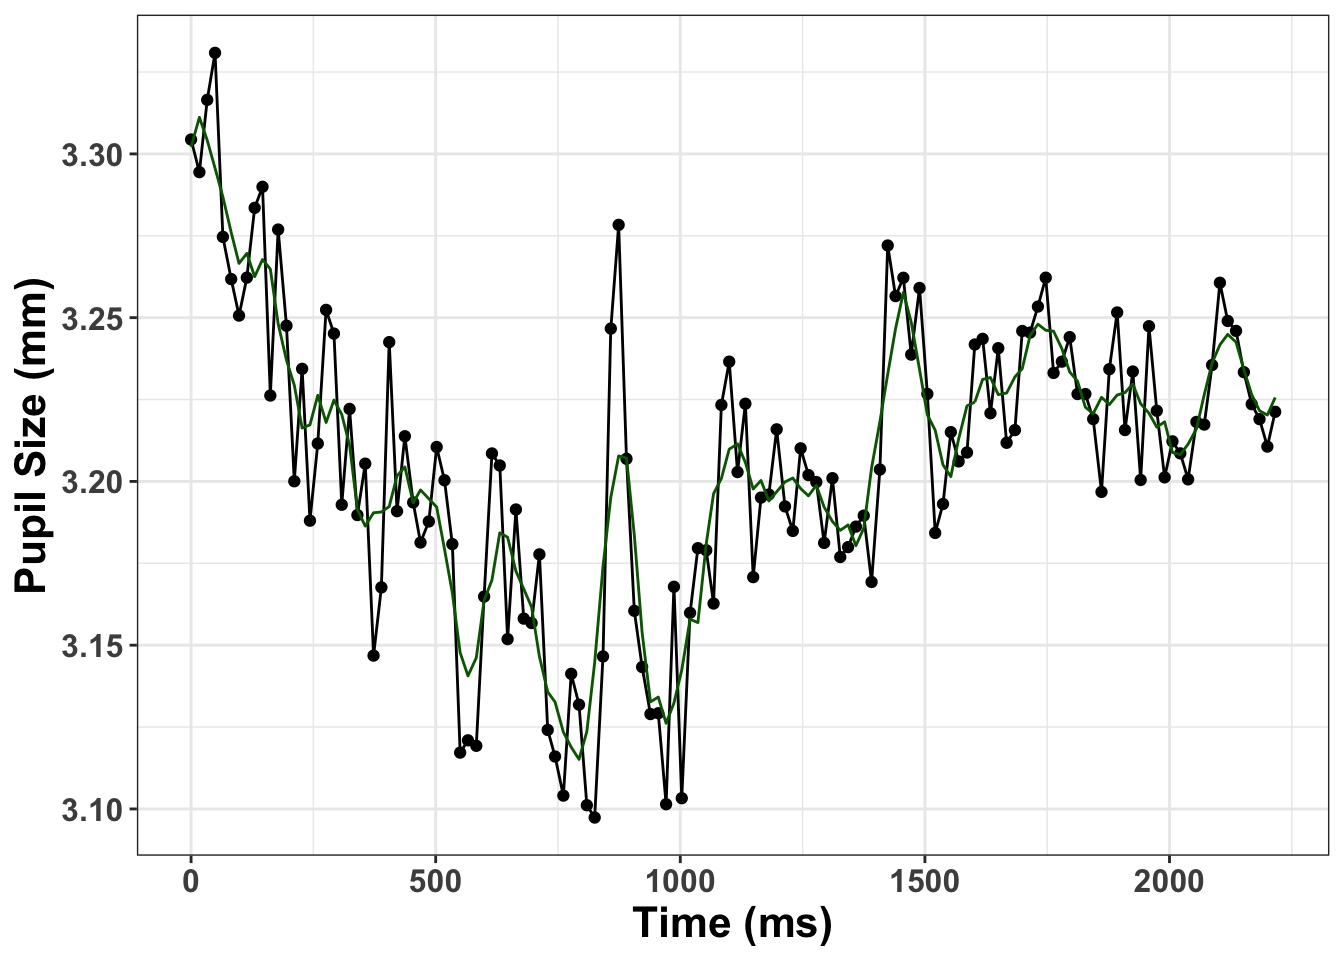
\includegraphics{gazepoint_files/figure-latex/unnamed-chunk-8-1.pdf}

\hypertarget{baseline-correction}{%
\section{Baseline Correction}\label{baseline-correction}}

Here we will do a subtractive baseline correction taking 250 ms before
the onset of the tone as baseline.

\begin{Shaded}
\begin{Highlighting}[]
\CommentTok{\#use messages to baseline correct}
\NormalTok{baseline\_pupil}\OtherTok{\textless{}{-}}\FunctionTok{baseline\_correction\_pupil}\NormalTok{(smooth\_interp, }\AttributeTok{pupil\_colname=}\StringTok{"pup\_interp"}\NormalTok{, }\AttributeTok{baseline\_window=}\FunctionTok{c}\NormalTok{(}\DecValTok{0}\NormalTok{,}\DecValTok{250}\NormalTok{), }\AttributeTok{baseline\_method =} \StringTok{"sub"}\NormalTok{)}

\FunctionTok{head}\NormalTok{(baseline\_pupil)}
\end{Highlighting}
\end{Shaded}

\begin{verbatim}
## # A tibble: 6 x 13
##   subject trial baseline  time pupil     x     y message tone  blink extendpupil
##     <dbl> <dbl>    <dbl> <dbl> <dbl> <dbl> <dbl> <chr>   <chr> <dbl>       <dbl>
## 1      13     1     4.80     0  4.80 -4.45 -14.1 START   lo        0        4.80
## 2      13     1     4.80    16  4.78 -4.45 -14.1 START   lo        0        4.78
## 3      13     1     4.80    32  4.79 -4.32 -13.7 START   lo        0        4.79
## 4      13     1     4.80    48  4.80 -4.58 -14.5 START   lo        0        4.80
## 5      13     1     4.80    64  4.80 -4.58 -14.5 START   lo        0        4.80
## 6      13     1     4.80    81  4.79 -4.63 -14.7 START   lo        0        4.79
## # ... with 2 more variables: pup_interp <dbl>, baselinecorrectedp <dbl>
\end{verbatim}

\hypertarget{missing-data}{%
\section{Missing Data}\label{missing-data}}

Let's see how much missing data there is and remove trials with greater
than 20\% missing data.

\begin{Shaded}
\begin{Highlighting}[]
\NormalTok{pup\_missing}\OtherTok{\textless{}{-}}\FunctionTok{count\_missing\_pupil}\NormalTok{(baseline\_pupil, }\AttributeTok{missingthresh =}\NormalTok{ .}\DecValTok{5}\NormalTok{)}
\CommentTok{\# remove outliers}
\end{Highlighting}
\end{Shaded}

I remove about 15 percent of trials.

\hypertarget{unlikely-pupil-sizes}{%
\section{Unlikely Pupil Sizes}\label{unlikely-pupil-sizes}}

Now let's keep pupil diameter sizes between 2 mm and 9 mm

\begin{Shaded}
\begin{Highlighting}[]
\NormalTok{pup\_outliers}\OtherTok{\textless{}{-}}\NormalTok{pup\_missing }\SpecialCharTok{\%\textgreater{}\%}
\NormalTok{  dplyr}\SpecialCharTok{::}\FunctionTok{filter}\NormalTok{ (pup\_interp  }\SpecialCharTok{\textgreater{}=} \DecValTok{2}\NormalTok{, pup\_interp }\SpecialCharTok{\textless{}=} \DecValTok{9}\NormalTok{)}
\end{Highlighting}
\end{Shaded}

\hypertarget{mad}{%
\section{MAD}\label{mad}}

Get rid of artifacts we might have missed during some earlier steps.

\begin{Shaded}
\begin{Highlighting}[]
  \CommentTok{\#MAD removal}
\NormalTok{max\_removal}\OtherTok{\textless{}{-}}\NormalTok{pup\_missing  }\SpecialCharTok{\%\textgreater{}\%}
\NormalTok{  dplyr}\SpecialCharTok{::}\FunctionTok{group\_by}\NormalTok{(subject, trial) }\SpecialCharTok{\%\textgreater{}\%}
\NormalTok{  dplyr}\SpecialCharTok{::}\FunctionTok{mutate}\NormalTok{(}\AttributeTok{speed=}\FunctionTok{speed\_pupil}\NormalTok{(pup\_interp,time)) }\SpecialCharTok{\%\textgreater{}\%}
\NormalTok{  dplyr}\SpecialCharTok{::}\FunctionTok{mutate}\NormalTok{(}\AttributeTok{MAD=}\FunctionTok{calc\_mad}\NormalTok{(speed)) }\SpecialCharTok{\%\textgreater{}\%}
\NormalTok{  dplyr}\SpecialCharTok{::}\FunctionTok{filter}\NormalTok{(speed }\SpecialCharTok{\textless{}}\NormalTok{ MAD)}
\end{Highlighting}
\end{Shaded}

\hypertarget{onset}{%
\section{Onset}\label{onset}}

Let's only look fron the start of the trial until 1500 ms

\begin{Shaded}
\begin{Highlighting}[]
\NormalTok{baseline\_pupil\_onset}\OtherTok{\textless{}{-}}\NormalTok{max\_removal }\SpecialCharTok{\%\textgreater{}\%}
\NormalTok{  dplyr}\SpecialCharTok{::}\FunctionTok{group\_by}\NormalTok{(subject, trial) }\SpecialCharTok{\%\textgreater{}\%}
\NormalTok{  dplyr}\SpecialCharTok{::}\FunctionTok{filter}\NormalTok{(time }\SpecialCharTok{\textless{}=} \DecValTok{1500}\NormalTok{) }\SpecialCharTok{\%\textgreater{}\%}
  \FunctionTok{select}\NormalTok{(subject, trial, time,baselinecorrectedp, tone, time,message,baselinecorrectedp)}
\end{Highlighting}
\end{Shaded}

\hypertarget{downsample}{%
\section{Downsample}\label{downsample}}

Downsample the time-course to 50 ms.

\begin{Shaded}
\begin{Highlighting}[]
\CommentTok{\#downsample}
\NormalTok{timebins1}\OtherTok{\textless{}{-}} \FunctionTok{downsample\_gaze}\NormalTok{(baseline\_pupil\_onset, }\AttributeTok{bin.length=}\DecValTok{50}\NormalTok{, }\AttributeTok{timevar =} \StringTok{"time"}\NormalTok{, }\AttributeTok{aggvars =} \FunctionTok{c}\NormalTok{(}\StringTok{"subject"}\NormalTok{, }\StringTok{"tone"}\NormalTok{, }\StringTok{"timebins"}\NormalTok{), }\AttributeTok{type=}\StringTok{"pupil"}\NormalTok{)}
\end{Highlighting}
\end{Shaded}

\begin{verbatim}
## Warning: The `.dots` argument of `group_by()` is deprecated as of dplyr 1.0.0.
## This warning is displayed once every 8 hours.
## Call `lifecycle::last_warnings()` to see where this warning was generated.
\end{verbatim}

\begin{Shaded}
\begin{Highlighting}[]
\NormalTok{timebins1}
\end{Highlighting}
\end{Shaded}

\begin{verbatim}
## # A tibble: 62 x 4
##    subject tone  timebins aggbaseline
##      <dbl> <chr>    <dbl>       <dbl>
##  1      13 hi           0    0.00130 
##  2      13 hi          50   -0.000752
##  3      13 hi         100   -0.00206 
##  4      13 hi         150    0.000331
##  5      13 hi         200    0.00530 
##  6      13 hi         250    0.00503 
##  7      13 hi         300    0.00826 
##  8      13 hi         350    0.00930 
##  9      13 hi         400    0.0116  
## 10      13 hi         450    0.0125  
## # ... with 52 more rows
\end{verbatim}

\hypertarget{visualize-time-course}{%
\section{Visualize Time-course}\label{visualize-time-course}}

\begin{Shaded}
\begin{Highlighting}[]
\NormalTok{cursive\_plot }\OtherTok{\textless{}{-}}\FunctionTok{ggplot}\NormalTok{(timebins1)}\SpecialCharTok{+}
  \FunctionTok{aes}\NormalTok{(timebins, aggbaseline, }\AttributeTok{linetype=}\NormalTok{tone, }\AttributeTok{color=}\NormalTok{tone) }\SpecialCharTok{+}
  \FunctionTok{stat\_summary}\NormalTok{(}\AttributeTok{fun =} \StringTok{"mean"}\NormalTok{, }\AttributeTok{geom =} \StringTok{"line"}\NormalTok{, }\AttributeTok{size =} \DecValTok{1}\NormalTok{) }\SpecialCharTok{+}
  \FunctionTok{theme\_bw}\NormalTok{() }\SpecialCharTok{+}
  \FunctionTok{labs}\NormalTok{(}\AttributeTok{x =}\StringTok{"Time (ms)"}\NormalTok{,}\AttributeTok{y =}\StringTok{"Pupil Dilation (baseline {-} pupil))"}\NormalTok{) }\SpecialCharTok{+}
  \FunctionTok{geom\_hline}\NormalTok{(}\AttributeTok{yintercept=}\FloatTok{0.0}\NormalTok{)}

\FunctionTok{print}\NormalTok{(cursive\_plot)}
\end{Highlighting}
\end{Shaded}

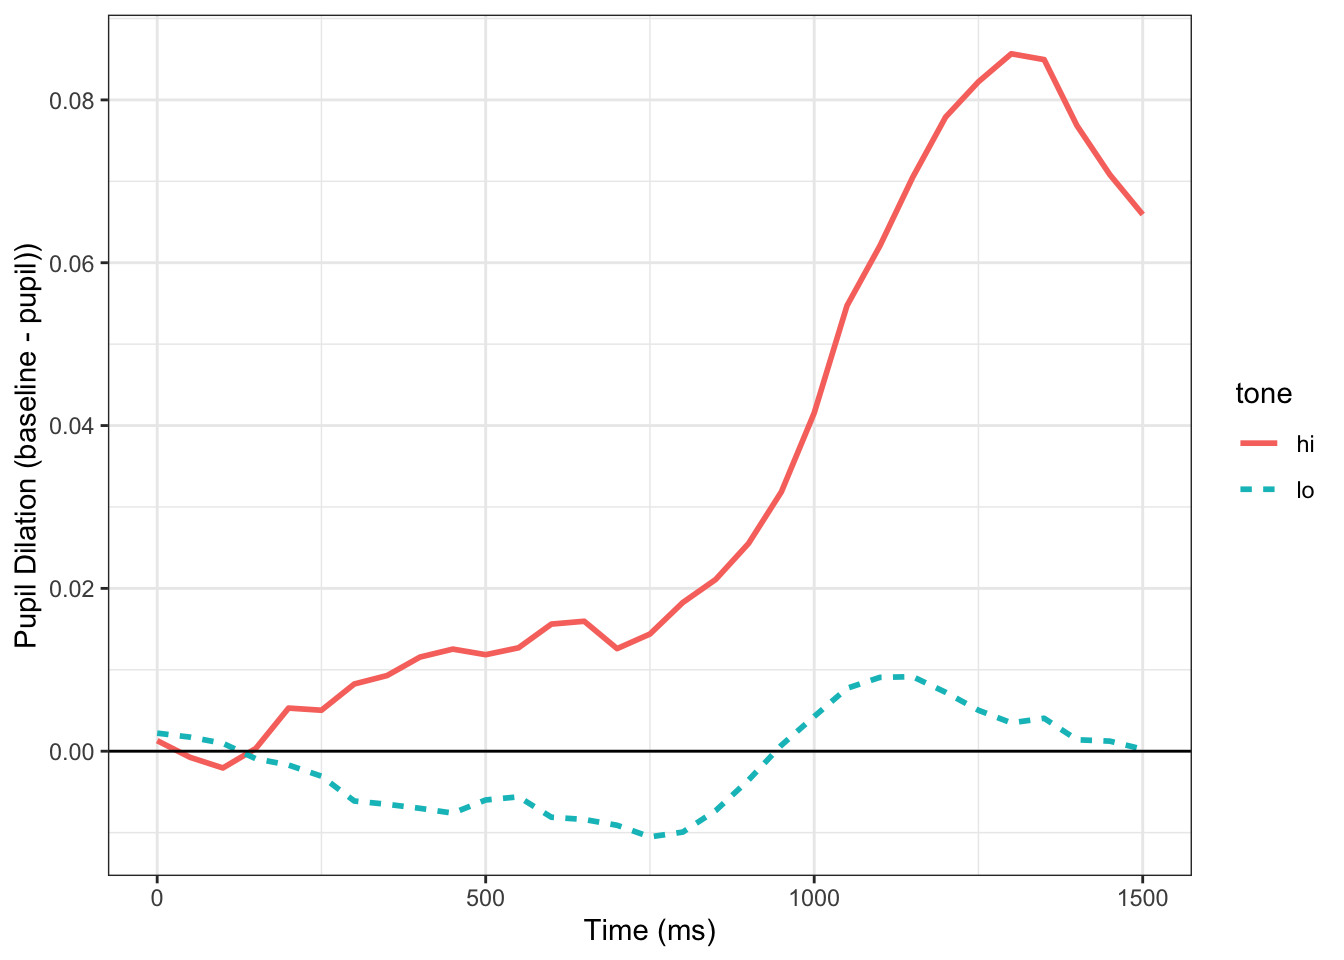
\includegraphics{gazepoint_files/figure-latex/unnamed-chunk-15-1.pdf}

This looks very similar to the one in the Tweet albeit a bit smoother as
a result of the extra preprocessing done.

\end{document}
